\documentclass[a4paper]{article}

\setcounter{tocdepth}{1}

\usepackage{color}
\usepackage{url}
\usepackage[T2A]{fontenc} % enable Cyrillic fonts
\usepackage[utf8]{inputenc} % make weird characters work
\usepackage{graphicx}
\usepackage{subcaption}
\usepackage{amsmath}
\usepackage{hyperref}


\usepackage[english,serbianc]{babel}

\usepackage[unicode]{hyperref}
\hypersetup{colorlinks,citecolor=green,filecolor=green,linkcolor=blue,urlcolor=blue}

\usepackage{listings}

\definecolor{mygreen}{rgb}{0,0.6,0}
\definecolor{mygray}{rgb}{0.5,0.5,0.5}
\definecolor{mymauve}{rgb}{0.58,0,0.82}

\lstset{ 
  backgroundcolor=\color{white},
  basicstyle=\scriptsize\ttfamily,  
  breakatwhitespace=false,         
  breaklines=true,                 
  captionpos=b,                   
  commentstyle=\color{mygreen},   
  deletekeywords={...},           
  escapeinside={\%*}{*)},          
  extendedchars=true,              
  firstnumber=1000,                
  frame=single,	                   
  keepspaces=true,                 
  keywordstyle=\color{blue},       
  language=Python,                 
  morekeywords={*,...},            
  numbers=left,                    
  numbersep=5pt,                   
  numberstyle=\tiny\color{mygray},
  rulecolor=\color{black},        
  showspaces=false,               
  showstringspaces=false,          
  showtabs=false,                  
  stepnumber=2,                   
  stringstyle=\color{mymauve},     
  tabsize=2,	                   
  title=\lstname                   
}

\begin{document}

\title{\Large Рибарење\\ \small{Семинарски рад у оквиру курса Основе математичког моделирања\\ Универзитет у Београду, Математички факултет}}

\author{Душан Пантелић\\ pantelic.dusan@protonmail.com}

\maketitle

\begin{center}
	
\includegraphics[width=3cm]{images/pmf.png}
\end{center}

\abstract{
Кроз овај рад читалац ће бити упућен у проблем рибарења, као и у математичко моделовање и решавање истог. Пре свега, шта представља проблем рибарења, његов значај, примену, али и проблеме при проналажењу оптимума и стања равнотеже модела. Представљене су формуле за одрећивање стања еквилибријума, и стања оптимума у зависности од различитих параметара модела. Читалац ће такође добити увид у графички приказ података на основу приказаног модела. На крају рада сумирани су закључци истраживања и изложени правци за даље истраживање и унапређивање.
\tableofcontents

\newpage

\section{Увод}
\label{sec:intro}
Математичким моделирањем рибарења за циљ имамо одређивање оптималног броја уловљене рибе у неком станишту тако да успоставимо равнотежу и не угрозимо опстанак рибе у том станишту, али и задовољимо потребе рибара. Решење горе наведеног проблема се користи и за одређивање квота тј. максималног дозвољеног броја уловљене рибе на неком подручју. Претпоставићемо да ограничен број ресусрса у станишту рибе утиче на величину популације рибе, а да је количина уловљене рибе пропорционална величини рибље популације. Нећемо узимати у обзир комплексније факторе као што су други предатори који такође лове рибу, економске факторе попут презасићења тржишта, понуде и потражње и друге.

\section{Популација рибе без рибарења}
\label{sec:nofishing}
За моделирање рибље популације без присуства рибара користићемо Верхулстов логистички модел.
\begin{equation}
    \label{nofishingeq}
    \frac{dN(t)}{dt} = rN(t)\left(1-\frac{N(t)}{K}\right)
\end{equation}
Из горе наведеног модела видимо да број рибе у неком трентку $N(t)$ зависи од стопе раста $r$, као и од оптималног броја рибе у станишту $K $ тако да има довољно ресурса за све. Решавањем овог модела добијамо следећу једначину:
\begin{equation}
    \label{nofishingeqsol}
    N(t) = \frac{N(0)e^r^t}{1+\frac{N(0)}{K}(e^r^t - 1)}
\end{equation}
Како би смо симулирали популацију рибе кроз време претпоставићемо да се риба налази у рибњаку и да су нам финансије ограничавајући фактор тако да максимално можемо купити хране за $10000$ риба што нам представља горе наведену константу $K$. Природни прираштај рибе од 30\% представићемо константом $r=0.3$, такође ћемо претпоставити да је постојало почетно улагање од 1000 риба што је почетна популација у рибњаку тј. $N(0)$. Симулацију броја рибе у наредних 50 година можемо видети на слици \ref{fishnofishing_view}. Mожемо приметити да након неког времена популација рибе тежи константи $K$, као и да прираштај нема ефекта због ограничења ресурса.
\begin{figure}[h!]
	\centering
	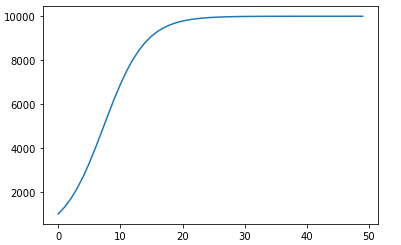
\includegraphics[width=10cm,height=3.5cm]{images/FishPopulationNoFishing.png}
	\caption{Популација рибе без рибарења}
	\label{fishnofishing_view}
\end{figure}


\section{Популација рибе са рибарењем}
\label{sec:fishingmodel}
Како би смо имали увид о популацији рибе приликом рибарења дефинисаћемо наредни модел (\ref{fishingmodeleq}) са пропорционалним рибарењем.
\begin{equation}
    \label{fishingmodeleq}
    \frac{dN(t)}{dt} = rN(t)\left(1-\frac{N(t)}{K}\right) - hN(t)
\end{equation}

\begin{itemize}
  \item $ rN(t)\left(1-\frac{N(t)}{K}\right)$ представља логистички модел дефинисан у претходном делу.
  \item $hN(t)$  представља количину уловљене рибе коју ловимо у неком временском периоду, где је $h$ интензитет риболова, а $N(t)$ тренутна популација рибе.
\end{itemize}
Диференцијалну једначину \ref{fishingmodeleq} можемо трансформисати у једначину \ref{eq2} сменама уведеним у \ref{eq1}. Приметимо да је новодобијена једначина иста као једначина \ref{nofishingeq} чије је решење \ref{nofishingeqsol} наведено у претходном делу, а сходно новим ознака добијамо \ref{eqsol1}, па заменом параметара добијамо решење диференцијалне једначине \ref{fishingmodeleq} приказано у \ref{eqsol2}

\begin{equation}
    \label{eq1}
    \left(A = r-h, B = \frac{K(r-h)}{r}\right)
\end{equation}

\begin{equation}
    \label{eq2}
    \frac{dN(t)}{dt} = AN(t)\left(1-\frac{N(t)}{B}\right)
\end{equation}

\begin{equation}
    \label{eqsol1}
    N(t) = \frac{N(0)e^A^t}{1+\frac{N(0)}{B}(e^A^t - 1)}
\end{equation}

\begin{equation}
    \label{eqsol2}
    N(t) = \frac{N(0)e^{(r-h)t}}{1+\frac{N(0)r}{K(r-h)}(e^{(r-h)t} - 1)}
\end{equation}

Нумеричка решења модела за параметре $[N(0)=[од 0 до 10000 са кораком 1000],  K=10000, r=0.5, h=0.25] $ можемо видети слици \ref{fishingmodel_view} која нам приказује промену величине популације рибе у периоду од 20 година.

 \begin{figure}[h!]
	\centering
	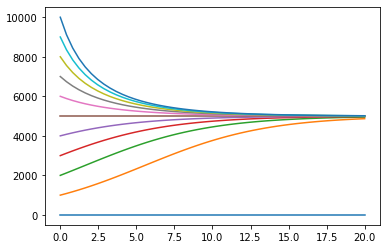
\includegraphics[width=10cm,height=5cm]{images/FishingModel.png}
	\caption{Популација рибе са рибарењем}
	\label{fishingmodel_view}
\end{figure}

 Можемо приметити да за све почетне популације рибе график тежи ка такозваним тачкама еквилибријума модела које доводе систем у стање равнотеже. Решавањем једначине \ref{fishingequilibrium} добијамо две тачке еквилибријума рибље популације које су приказане на \ref{fishingequilibriumsol}.

\begin{equation}
    \label{fishingequilibrium}
    rN\left(1-\frac{N}{K}\right) - hN = 0
\end{equation}

\begin{equation}
    \label{fishingequilibriumsol}
     \left(E1 = 0,   E2 = \frac{K(r - h) }{r}\right)
\end{equation}

Када убацимо параметре из нумеричког приказа модела са слике \ref{fishingmodel_view} у формуле за тачке еквилибријума \ref{fishingequilibriumsol}, добијамо вредности $(E1=0, E2=5000)$. Видимо са графика да популација рибе зависно од почетне вредности тежи једном или другом еквилибријуму, када број рибе достигне еквилибријум он се више не мења и систем улази у стање равнотеже.Такође из формуле за тачке еквилибријума видима да уколико је интензитет риболова $h$ већи или једнак стопи раста рибље популације $r$, друга тачка еквилибријума постаје $E2=0$ јер иако генерално можемо имати негативан еквилибријум он нема смисла јер никада не можемо имати негативну популацију рибе већ негативност можемо интерпретирати као брзину пада ка 0. На слици \ref{equilibriumsgraph} можемо видети како се мењају тачке еквилибријума са променом интензитета риболова за фиксну стопу раста од 0.5.

\begin{figure}[h!]
	\centering
	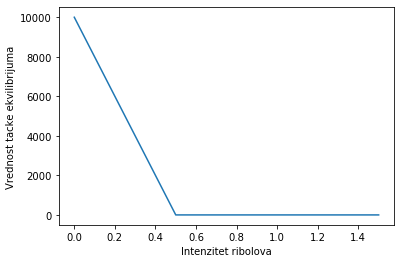
\includegraphics[width=10cm,height=5.0cm]{images/Equilibriums.png}
	\caption{Еквилибријуми у зависности од интензитета риболова}
	\label{equilibriumsgraph}
\end{figure}

Примећујемо да се вредност тачке еквилибријума смањује линеарно са порастом интензитета риболова. За $r>h$ еквилибријум $E1=0$ је нестабилан јер за било који почетну популацију већу од нуле тежимо еквилибријуму $E2$ добијеном по формули који је стабилан за претпостављени однос $r>h$. Уколико је $r \leq h$ еквилибријум $E1=0$ постаје стабилан и за све почетне попилације рибе тежимо ка њему, а еквилибријум $E2$ постаје негативан, а самим тим и недостижан и нестабилан.

\section{Оптимална количина уловљене рибе}
\label{sec:fishingoptimum}
Како би наш претходно дефинисани модел у пракси био одржив на дужи временски период потребно је успоставити равнотежу између броја рибе у станишту и количине уловљене рибе у зависности од вредности параметара модела. Не желимо прекомерну количину рибе која ће умирати због недостатака ресурса, али такође не желимо ни превелику количину уловљене рибе која ће можда истребити рибу.

За проналазак оптималног случаја користиће нам стања равнотеже модела тј. еквилибријуми. Како смо видели да популација рибе тежи еквилибријуму на дужи временски период посматраћемо количину уловљене рибе у односу на достигнути еквилибријум, при чему еквилибријум у $0$ нећемо користити. 
Ако количину уловљене рибе означимо са $Y = h*N$ заменом количине рибе $N$ са количином рибе у еквилибријуму из формуле добијамо једначину \ref{maxyeald} чији максимум тражимо у нули извода \ref{yielddiff} по $h$.
\begin{equation}
    \label{maxyeald}
    Y = h*\frac{K(r - h) }{r}
\end{equation}

\begin{equation}
    \label{yielddiff}
     \frac{dY}{dh} = -\frac{K(2h - r) }{r}
\end{equation}

Решавањем нуле извода \ref{yielddiff} добијамо максималну количину уловљене рибе за интензитет риболова $h=\frac{r}{2}$. Применом претходно добијене формуле за $h$ добијамо да је тачка еквилибријума $E=\frac{K}{2}$ а количина уловљене рибе $Y=\frac{Kr}{4}$. 

\begin{figure}[h!]
	\centering
	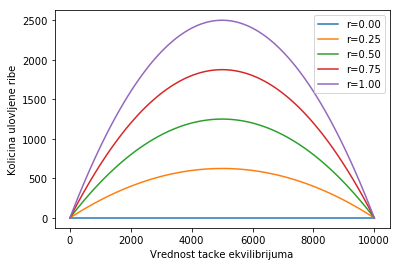
\includegraphics[width=10cm,height=5.0cm]{images/OptimalHarvest.png}
	\caption{Почетни еквилибријум}
	\label{optimalHarvest}
\end{figure}


На слици \ref{optimalHarvest} видимо график који нам приказује количину уловљене рибе у односу на вредност тачке еквилибријума за различите стопе раста рибље популације $r$. Како нам је вредност $K=10000$ са графика можемо видети да максимуме стварно добијамо у тачкама еквилибријума $E=\frac{K}{2}=5000$. Такође видимо да је максималан улов стварно добијен по формули $Y=\frac{Kr}{4}$, и да директно зависи од стопе раста $r$ што се испољава већим максимумима на функцијама са већом стопом раста. Интензитет риболова $h$ смо рачунали на основу $r$ и $K$ тако да модел буде у стању равнотеже, док ћемо у наредном делу видети како промена интензитета риболова утиче на количину уловљене рибе.


\section{Количина улова у односу на интензитет риболова}
\label{sec:fishingintensity}
 Видели смо да у претходном поглављу да нам је један од најинтересантнијих параметра модела интензитет риболова, јер у некој реалној ситуацији тај параметар можемо да контролишемо док капацитет природног станишта и прираштај рибе не можемо. У овом делу ћемо помоћу експерименталних резултата продискутовати како промена интензитета риболова утиче на количину уловљене рибе. На сликама \ref{intensityincrease1} и \ref{intensityincrease2} можемо видети како се мења просечна количина уловљене рибе са променом интензитета риболова за редом почетне популације рибе од 100 и 10000, такође смо приказали графике за различите вредности стопе раста рибље популације.
 
\begin{figure}[h!]
	\centering
	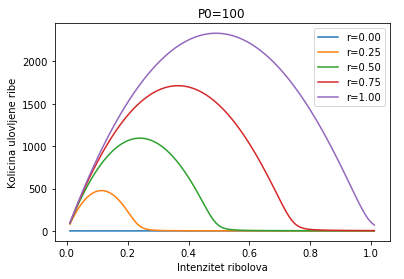
\includegraphics[width=10cm,height=4.0cm]{images/IntenzityChangeP100.png}
	\caption{Однос уловљене рибе са променом интензитета риболова 1}
	\label{intensityincrease1}
\end{figure}
 
 \begin{figure}[h!]
	\centering
	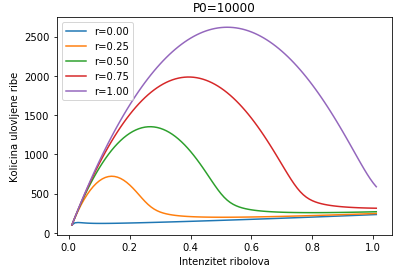
\includegraphics[width=10cm,height=4.0cm]{images/IntenzityChangeP10000.png}
	\caption{Однос уловљене рибе са променом интензитета риболова 2}
	\label{intensityincrease2}
\end{figure}

Са горе поменутих слика видимо да избор почетне популације рибе врло мало утиче на резултате и да су резултати скоро идентични за дужи временски период, чиме смо потврдили да за дужи временски период оптималан улов можемо посматрати на основу еквилибријума ка којима модели теже. Примећујемо да са порастом интензитета риболова расте количина уловљене рибе до неке тачке максимума након чега креће опадање и евентуално истребљење рибе, а самим тим и количина уловљене рибе тежи нули. Са графика можемо видети да је малопре поменута тачка максимума за $h=\frac{r}{2}$ што се слаже са резултатима добијеним у претходном делу, и да свако одступање од оптималног интензитета риболова доводи до смањења количине уловљене рибе.

\section{Закључак}
\label{sec:final}
Представили смо математички моделом за популацију рибе са пропорционалним риболовом, а затим смо продискутовали стања равнотеже модела. Закључили смо да ће након неког временског периода популација рибе ући у еквилибријум и да за даље истраживање можемо користити тачке еквилибријума без губитка општости. На основу еквилибријума модела пронашли смо везу између интензитета риболова и оптималне количине уловљене рибе, али и параметара попут стопе раста рибље популације и капацитета природног станишта на које не можемо утицати у неким реалним ситуацијама. Такође смо посматрали промену уловљене рибе са променом интензитета риболова чиме смо потврдили претходно добијене резултате за оптимални интензитет риболова. 

\nocite{mathmodeling}
\nocite{fishhavresting}
\nocite{fishanalysis}
\nocite{predatory}
\nocite{optimalhavrest}
\nocite{fishingstrategies}
\nocite{limitedgrowth}
\nocite{harvestmodel}

\addcontentsline{toc}{section}{Литература}
\appendix
\bibliography{Fishing} 
\bibliographystyle{plain}
\end{document}
